\documentclass[12pt]{report}
\usepackage{WUbiblio,WUthesis}
%\usepackage[latin1]{inputenc}
\usepackage{amsmath}
\usepackage{amsfonts}
\usepackage{amssymb} 
\usepackage{graphicx}
\graphicspath{ {images/} }
\usepackage{listings}
\usepackage{minted}
%\usepackage[revision]{revann}
\usepackage{tikz}
\usepackage{array}
\usepackage{subcaption}
\begin{document}

\title{Photometry of Celestial Fireballs Using a Portable All-Sky Camera}
\author{Luke Galbraith Russell}
\thesissupervisor{Dr. Jed Rembold}

\maketitle


\newpage

\begin{center}
\textbf{Presentations and publications}

Poster??
\bigskip

L. Russell, Photometry of Celestial Fireballs, Oral Presentation at Willamette University, SSRD (April 2018)
\bigskip

L. Russell, Photometry of Celestial Fireballs, Oral Presentation at Willamette University, Research Seminar I: Status Report Presentation (December 2017)
\bigskip

L. Russell, Photometric Analysis of Earthbound Fireballs, Oral Presentation at Willamette University, Advanced Techniques in Experimental Physics: Senior Proposal Presentation (March 2017)
\bigskip
\end{center}



\begin{acknowledgments}
I would like to thank the following professors for writing me letter of recommendations and for their own respective contributions:
\begin{itemize}
	\item Dr. Jed Rembold for dealing with all my stupid questions regarding life and this thesis.

	\item Dr. Rick Watkins for being pretty dang funny.

	\item Dr. Daniel Borrero for forcing me in class to \textit{explain} code instead of just turning it in.

\end{itemize}
I would also like to thank the following people for being pretty swell and whatnot.

\begin{itemize}
	\item Adam Newton Wright for his future contributions on our Nobel Prize-winning discoveries, as one can never have too many gold-plated coasters.

	\item Kelsey Walker for having optimism so bright it would immediately oversaturate our all-sky camera's sensors.

	\item Mark Watney for making all my problems seem lame.

	\item All the angels on Stack Overflow who spend their time answering weirdly specific coding questions that I end up looking at years later.
\end{itemize}

\end{acknowledgments}

\begin{abstract}
\section*{General Abstract}
We do not want valuable technology we send out in space to be destroyed by the population of rocks surrounding Earth. Therefore, it is important to know exactly how many rocks are out there and how big they are. Our portable video camera device can detect and then record the rocks burning up in Earth's atmosphere. This project focuses on writing software to see how bright those rocks are based off of the video collected by the device. The brightnesses can be used later to estimate their sizes.

\section*{Technical Abstract}
When designing new satellites, incorporating damage mitigation techniques is currently difficult due to a lack of understanding about the near-Earth small asteroid population. In an effort to investigate this population, we have constructed a portable all-sky camera to continuously monitor the night sky. It has the capability to detect meteors ablating in Earth's atmosphere and record their brightness as pixel values. To begin to measure the number and size distribution of the meteoroids that later became these meteors, this project focuses on writing software to automatically measure a meteor's brightness, and  calibrate it to a known astronomic luminosity, which can later be used to estimate its size. When ran on videos from NASA, The program produced similar light curves to theirs, showing a strong proof of concept.

\end{abstract}

\tableofcontents
\listoftables
\listoffigures

\chapter{Introduction}

Space, while mostly space, is not entirely empty.  There are planets, stars, comets, and many other objects, but here we are concerned about meteors. Specifically, we are interested in the smallest meteors. While rocks the size of pebbles may not seem dangerous to those of us protected by Earth's atmosphere, they pose a great threat to equipment and life beyond our atmosphere. We desire to know how many of these objects are in orbit near Earth in order to estimate the necessary level of protection for our structures and to better estimate the lifespans of our structures.

Currently, one of the ways meteors can be detected entering our atmosphere is by all-sky cameras detecting the bright streaks they leave as they ablate in the atmosphere. This brightness is what gives them another name: fireballs. All-sky cameras are set up by NASA and other groups\cite{Jenniskens2011,Trigo-Rodriguez2007}. They are installed on roofs or mounts and hooked up to desktop computers in buildings. It is a big and inflexible setup. This large setup limits the amount of setups that currently exist, which in turn limits the amount of total sky coverage we can get. Our all-sky camera explores a new design: one in which its detection software is housed inside its small, basketball-sized chassis. It still depends on external power, but low power consumption makes it a strong candidate to run off battery power if needed. We aim to show that our tiny unit (named D6\footnote{D6 is named after a droid in the Star Wars universe similar to R2-D2, but is green and owned by Wedge Antilles.}) is capable of observing and analyzing fireballs just as reliably as the larger, more established networks .

We are using our all-sky camera to detect meteors and then implementing photometry to calculate the meteors' magnitudes, then extrapolating their masses from those magnitudes. There have been many other studies by larger all-sky networks to create a model for the population distribution. We have no reason to expect our data to deviate greatly from this trend. In fact, we are hoping to test the effectiveness of our all-sky camera setup by comparing its findings to the established model. Also, while the general trend is well known, there is no guarantee that it is as precise as it could be. We are curious about any possible small discrepancies within the model regarding the smaller size meteoroids, and believe that if any discrepancies are there, they would only become apparent if data was being collected much more frequently than the current rate.

The background section details the information needed to understand what fireballs are and why they are important. The size of a meteor is determined through a long chain of physical relations that begin at its apparent magnitude, and is explained in detail in the methods section. The actual results are then presented in the data section.


\chapter{Background}
With respect to the Sun, our planet is moving through space at 30 kilometers per second. Many other objects orbit the sun, and those orbits can overlap or nearly overlap Earth's. The vast majority of these objects are small and are difficult to detect. These objects are known as near-Earth objects. Near-Earth objects consist of many similar rocks, but they have important differences between them. Regardless, they are hazards of the solar system, so we use systems such as all-sky cameras to detect them and gather data about their population distribution.

\section{Asteroids and Meteoroids}
There are five terms that are often incorrectly used interchangeably to describe rocks from space. They are the following: asteroid, meteoroid, meteor, meteorite and fireball. They are visually represented in Figure~\ref{fig:neos}. It should be noted that a comet does not belong with these terms as only a small percentage of a comet's composition is rock: it is a mass of ice and dust. Compositionally, asteroids and meteoroids are the same. They are composed of rock or metal and travel through space outside Earth's atmosphere. They are delineated by their size.  In order to be defined as a meteoroid, the piece of rock should be at least \mbox{100 $\mu$m}\footnote{Anything smaller than this is nothing more than dust, which makes up the interplanetary dust cloud.}\cite{Steel1996}. The accepted upper boundary on what constitutes a meteoroid but not an asteroid is around 10 meters. 
Asteroids are much larger, such as the asteroid that caused the Chicxulub crater in the Yucatan peninsula \cite{Bottke2007}.

In terms of their origins, meteoroids are often fragments of asteroids that are separated by some sort of collision in space, or are small pieces of rock and dust that are left behind by comets. Near-Earth asteroids are most likely objects expelled from the main asteroid belt between Mars and Jupiter due to Yarkovsky thermal forces or secular resonances \cite{Bottke2007}. The Yarkovsky thermal force is a net force that occurs from the heating up of one side of an asteroid or meteoroid from the sun. The hotter side dissipates more energy while cooling than the already cold side, and thus that departing energy results in a recoil force moving the asteroid in the direction opposite the hotter side \cite{Bottke2006}. Secular resonance is when an asteroid syncs its precession to a nearby planet. This disturbs the orbit of the asteroid, and causes it to slowly change its orbital eccentricity as a result \cite{Moons1995}.

\begin{figure}[ht!]
  \centering
  \includegraphics[scale=.2]{neos.png}
  \caption{A visual representation of the different varieties of rock in the space near Earth (Photo courtesy of Dr. Jed Rembold).}
  \label{fig:neos}
\end{figure}


\section{Fireballs and Meteors}

Asteroids and meteoroids are by definition only found outside the atmosphere of the planet. They becomes meteors only when they enter the atmosphere. Some literature even rechristens their status from near-Earth objects to inside-Earth objects, or IEOs for short \cite{Bottke2007}. Fireballs are especially bright meteors, and are often chosen to be studied due to their comparatively easy detection. Technically, fireballs are only considered such if they are brighter than Venus, with a magnitude of around -4, but the colloquial use is much less stringent \cite{Harbaugh2008}. 

Most of the time, meteors are completely destroyed as they travel through the atmosphere. This is done through ablation due to how they interact with molecules in the atmosphere. As the meteor hits the molecules in the atmosphere, ionization occurs. The point in the atmosphere at which light is emitted varies based on the velocity of the object. Slower objects need to be in a denser part of the atmosphere before ablation can occur. The average point at which this happens is most often between 70 and 110 kilometers above sea level \cite{Halliday1996}. During this process the meteor loses mass and energy in the form of light. The percentage of energy converted to life is known as the luminous efficiency and is an important term in predicting the mass of a meteor from its luminosity. If there is still mass remaining by the time it comes into contact with the Earth, it cools and becomes a meteorite. More often than not, however, meteors are vaporized tens of kilometers above sea level \cite{Halliday1996}.

Meteors tend to appear during two types of events. The first event is a meteor shower and can be reliably predicted. This is due to Earth going through parts of space where known debris are located. The debris are trails left behind by comets. The majority of these comet trails are due to water vapor drag. As a comet moves around the sun, different parts of its ice evaporate, freeing the small pieces of rock that were embedded inside it \cite{Whipple1951}. A meteor shower can also be caused by a large amount of debris left behind when a comet is fragmented in space \cite{Jenniskens2006}. Many meteor showers are well charted and known at this point. As of this writing there are 112 established meteor showers, with the potential of hundreds more \cite{RRudawskaZKanuchova2017}. Besides a meteor shower, the other event is a single isolated event, called a sporadic event. A sporadic event may have originally been part of a meteor shower or an asteroid belt before getting set off course due to extraneous forces.

\section{Near-Earth Objects}
While there are differences between the types of near-Earth objects, they all share one thing in common: they pose a hazard to any sort of human structure sent out into space. Having more accurate and complete data on the population of these objects will give humanity a better chance to adequately defend these structures and shelters as well as more accurately estimate their lifespans. As space exploration develops, this will become more relevant, with potential landing spots for humans on the Moon and on Mars not having the luxury of the protective atmosphere of Earth. This can be seen just by looking up at the night sky; the moon is pockmarked with craters. This is not just exclusive to the moon, as craters can be seen on any rocky space object that does not have a thick atmosphere. These craters are the most obvious pieces of evidence of meteor strikes The moon also provides another strong example of the power of these strikes, as when a meteoroid hits the lunar surface, enough energy is released as to be visible from Earth \cite{Rembold2015}. Without the protective atmosphere, near-Earth objects could potentially wreak havoc on any structures. For example, the European Space Agency communication satellite Olympus was permanently decommissioned due to damage sustained during the Perseid meteor shower of 1993. The majority of international and national organizations\footnote{These include, but are not limited to, the United Nations, the United States Congress, the European Council, the UK Parliament, the IAU, OECD, NASA, and ESA\cite{Bottke2007}} concerned with planetary protection have all deemed large near-Earth objects to be credible threats to Earth and to any missions out of its atmosphere\cite{Bottke2007}.

Observational data from many different studies has resulted in a model for the population distribution of these objects. Specifically, there is a well-known linear relationship between the mass of an asteroid and the number that exist if plotted along log-log axes \cite{Rembold2015}. This is shown in Figure \ref{fig:population}.

\begin{figure}[ht!]
  \centering
  \includegraphics[scale=.5]{population.png}
  \caption{The population distribution of near-Earth objects is straightforward: small objects are often much more likely than large objects. \protect\cite{Rembold2015}}
  \label{fig:population}
\end{figure}

Initially this model seems reassuring. The larger objects, which would have the most  potential to cause damage, are much less common than the smaller, less energetic objects. This can be seen in Equation \ref{eq:ke}, where $m$ is equal to the mass and $v$ is equal to the velocity of the object.
\begin{equation} \label{eq:ke}
	\textrm{Kinetic Energy} = \frac{mv^2}{2}
\end{equation}
However, these small objects still pose a large threat to structures due to their extremely fast velocities. A one-millimeter meteoroid has similar strength to a 22-caliber bullet, while a one centimeter meteoroid can be as powerful as a cannonball. This is because velocity is the dominant term in equation \ref{eq:ke} and meteoroid speeds can range from 11 to 70 kilometers per second \cite{Harbaugh2008}. Figure \ref{fig:damage} shows the damage that a pebble-sized object can do to a thick slab of metal, and satellites without armor are much more fragile than that.

\begin{figure}[ht!]
  \centering
  \includegraphics[width=10cm]{damage.jpg}
  \caption{Even small objects such as this ball bearing can exert tremendous amounts of force if they are traveling at 50 kilometers per second \protect\cite{ESA2017}.}
  \label{fig:damage}
\end{figure}


It should be noted that while this model appears consistent, and it may very well be, it is not guaranteed. With such a high population of smaller-sized objects, any variance could greatly change the likelihood of accurately accounting for potential damage. For instance, a satellite can only take so many impacts with meteoroids before becoming disabled. Even if there are only slightly more meteoroids than currently predicted, the lifespan of that satellite would be shortened, jeopardizing missions. 

\section{Detecting Fireballs}
There are many current projects aimed at collecting optical data about meteors \cite{Jenniskens2011,Trigo-Rodriguez2007,Halliday1996}. Most make use of all-sky cameras. All-sky cameras are CCD cameras that are often utilized as video capture devices, recording either 25 or 30 frames per second depending on its video signal \cite{Molau2005}. An all-sky camera is a camera that provides a view of up to 180$^{\circ}$ of the sky above, producing a circular image, as seen in Figure \ref{fig:skypic}. This allows a clear view of the sky as a whole, allowing for easy identification of constellations. By locating constellations, stars can be identified and objects can have their relative location recorded. 
\begin{figure}[ht!]
  \centering
  \includegraphics[width=10cm]{skypic.png}
  \caption{All-sky cameras feature a 360$^{\circ}$ view of the horizon, providing maximum sky coverage. This is an image from a high resolution color camera \protect\cite{Alcor}.}
  \label{fig:skypic}
\end{figure}

In reality, this view is not quite 180$^{\circ}$, but more often around 140$^{\circ}$ due to the fact that lenses wide enough to take in 180$^{\circ}$ end up just taking in the edges of the all-sky cameras chassis instead. Our own camera is only able to see 140$^{\circ}$ into the sky. Figure \ref{fig:atmosphere} shows how much of the sky is covered. The amount of Earth being covered is defined by taking the edges of the all-sky camera view and treating those as zeniths. A zenith is the point in the sky that is directly above a certain point on Earth. Those points on Earth are the edges of how much of the Earth it covers. Knowing how much of the Earth is covered is useful because those zeniths provide the points where another camera can be placed to overlap one half of the original camera's view of the sky. Overlapping is useful because multiple camera angles allow the triangulation of the object's position and velocity. The amount of sky coverage can be found through trigonometry, resulting in equation \ref{eq:coverage}, where $\Omega$ is the steradian, $h+r$ is the distance from the center of the Earth to the edge of the area of sky coverage, and sr is the unit steradian.
\begin{figure}[ht!]
	\centering
	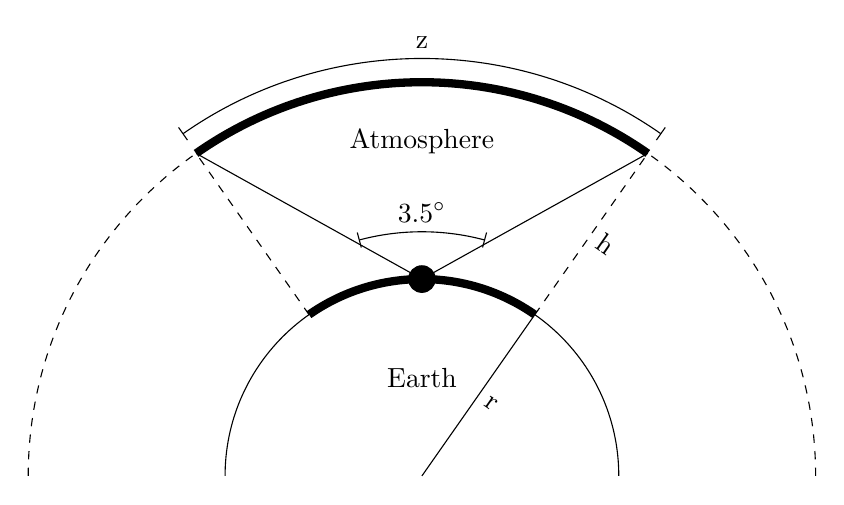
\begin{tikzpicture}
		\draw (0:2.5) arc (0:180:2.5) node at (0,1.25) {Earth};
		\draw[dashed] (0:5) arc (0:180:5) node at (0,4.25) {Atmosphere};
		\draw[] (0,0) -- (55:2.5) node[midway,right,sloped,rotate=270] {r};
%		\draw[dashed] (0,0) -- (125:4);
		\draw (0,2.5) -- (55:5);
		\draw (0,2.5) -- (125:5);
		\draw[dashed] (125:2.5) -- (125:5);
		\draw[dashed]  (55:2.5) -- (55:5) node[midway,right,sloped,rotate=270] {h};
		\draw[line width=3pt] (55:2.5) arc (55:125:2.5);
		\draw[line width=3pt] (55:5) arc (55:125:5);
		\draw[|-|] (55:5.3) arc (55:125:5.3) node[midway,above] {z};
		\draw[|-|] (75:3.1) arc (75:105:3.1) node[midway,above] {$3.5^{\circ}$};
		\fill (0,2.5) circle [radius=5pt];
	\end{tikzpicture}	
	\caption{The all-sky camera can see distance $z$. The area of the Earth it covers are between the points that have the endpoints of $z$ as their zeniths along height $h$. Note that the height of the atmosphere where ablation occurs is often less than 100 kilometers, while the radius of the Earth is 6,371 kilometers, so the radii are not to scale.}
	\label{fig:atmosphere}
\end{figure}


\begin{equation} \label{eq:coverage}
	\textrm{Sky Coverage} = \Omega(h+r)^2
\end{equation}

Using an average height $h$ of 75 kilometers, the area of the sky that is covered by an all-sky camera such as ours is around 119,000 square kilometers. This is equal to 118,000 square kilometers of land coverage. This is only 0.023 percent of the Earth that is covered, so there is a need for more all-sky cameras to ensure better coverage. Our all-sky camera has been in two locations, Salem and Baker City, Oregon. These two spots provide examples of how much land can be covered in Figure \ref{fig:coverage}. Even for two locations in the same state, there is no overlap.

\begin{figure}[ht!]
	\centering
	\includegraphics[width=10cm]{coverage.png}
	\caption{An all-sky camera can cover a circle with a radius of roughly 200 miles.}
	\label{fig:coverage}
\end{figure}


All-sky cameras are currently detecting fireballs in many places around the world. One notable example is NASA's Camera for All-Sky Meteor Surveillance (CAMS) Network. They have cameras located throughout many parts of the United States, forming a strong cohesive network. The CAMS network has been successful in correctly detecting all known meteor showers\footnote{The meteor showers were the theta Aurigids, chi Taurids, omicron Eridanids, and the supposed iota November Aurigids. The latter was in fact shown to be merely an overlap between the theta Aurigids and chi Taurids with CAMS network data.} during the month of November in 2011\cite{Jenniskens2011}.

NASA is not the only one to have such a network, with other organizations such as the SPanish Meteor Network (SPMN) also possessing well established systems of their own. They were  able to successfully confirm expected meteor showers with the use of their high-resolution, all-sky cameras.\footnote{The meteor showers were the Orionids, the Taurid stream related to comet 2P/Encke, and the delta Aurigids.} They even were able to find the nu Aurigids, that while previously identified, were not expected to be seen \cite{Trigo-Rodriguez2007}. These organizations are able to collect large amounts of data with all-sky camera networks compared to previous endeavors but they do not have enough cameras to come even close to covering the entire sky. Figure \ref{fig:network} shows the Sky Sentinel Camera Network and their coverage in the United States. The network currently operates a network of around 65 cameras and hope to have over 100 in the future \cite{Bannister2012}.

The current model is to have these cameras connected to large structures or buildings with desktop computers where they can access the constant power and internet access that is needed for the detection and analysis. The necessary infrastructure that is currently needed lends these networks to be built in more urban areas, where light and air pollution become more problematic. Therefore this  model also severely limits not only the quantity of skies covered, but also the quality.

\begin{figure}[ht!]
	\centering
	\includegraphics[width=10cm]{network.png}
	\caption{This network manages to cover a lot of area, but it may not have the best observational quality due to the cameras being centered in cities \protect\cite{SkySentinel}.}
	\label{fig:network}
\end{figure}

All-sky cameras themselves are not inherently complex. They are small and can be built relatively cheap, with builds being found online from Sky at Night Magazine and New Mexico State University, among others \cite{Bannister2012}. Figure \ref{fig:schematic} shows the diminutive size of a camera used by the Sky Sentinel network, but also shows the power and video signal cords that have to connect to an external desktop for analysis. 

Having a small, portable system has many potential benefits. Not only does a portable system increase ease of use and decrease equipment cost, it also vastly improves flexibility. For example, if nearby blooming trees block some view of the sky during the spring, a portable system could just be moved, while a permanent system would require the removal of the trees or the acceptance of a less than optimal observational status.

\begin{figure}[ht!]
	\centering
	\includegraphics[width=10cm]{schematic.png}
	\caption{This schematic of an all-sky camera leaves out the attached structure to which the bottom cords must connect\protect\cite{Bannister2012}.}
	\label{fig:schematic}
\end{figure}

Software accompanies all-sky camera systems to perform meteor detections. This saves the user from having to watch hours of video looking for events that may just be a few seconds long. Detection systems look for moving patches of light, and thus can produce numerous false positives from other environmental factors. These include light being reflected off moving clouds and planes flying through the field of vision \cite{Harbaugh2008}. Fortunately, these false positives can mostly be eliminated by visual inspection. The exact setup depends on the specific system, but meteor detection is either constantly processed by a computer checking the frames as they arrive, or the video is stored as a whole to be run through a detection program at a later date \cite{Molau2005}. The software is full-fledged but bulky as a result. For example, METREC is a meteor detection software that is used by networks such as the Polish fireball network. It requires a desktop computer to operate\cite{Molau2005}. The hardware requirements thus require a complete computer to accompany the camera.  

\section{Analyzing Fireballs}

An all-sky camera can result in the acquisition of many pieces of useful information about a meteor. That being said, there are parameters a single all-sky camera cannot extract that a full network can, such as velocity and height. If there is a system of multiple cameras detecting the same meteor the orbit can be extrapolated as well \cite{Trigo-Rodriguez2009}. The Canadian fireball network detected 259 fireballs in 1996, and was able to get values for height, velocity, magnitude and mass for every fireball \cite{Halliday1996}. A single all-sky camera would only be able to get magnitude, and would have to extract mass from that. For a full fireball network, having velocity means it can find the mass using equation \ref{eq:mass}, where $m_d$ is the mass at a certain point in the flight, $A$ is the cross sectional area at that same point in flight, $\rho_a$ is the atmospheric density, and $v$ is velocity \cite{Halliday1996}.

\begin{equation} \label{eq:mass}
	\frac{m_d}{A} = -\frac{\rho_a v^2}{2 \dot v}
\end{equation}

Not only does the velocity help determine mass in this situation, it also can be used to work backwards to find an estimate of the velocity before the affects of drag began slowing it down. This means that all-sky cameras can be used to gather data on the potential velocities of meteor showers in open space. The SPanish Meteor Network (SPMN) used velocity data to extrapolate such pre-atmosphere velocities with their five station setup in 2006 \cite{Trigo-Rodriguez2007}. 

Ultimately, all-sky cameras are most useful for measuring the photometric qualities of objects in the sky. They can detect fireballs and then provide the needed data to determine the fireballs' magnitudes, which is how bright they appear to the camera. This, however, can be done with just a single all-sky camera.

It should be noted that there are differing techniques when performing photometry. Different cameras are more sensitive to different wavelengths of light, and that can make comparing results from different cameras challenging. One solution to this is to apply a filter. A filter isolates light along a specific wavelength of the electromagnetic spectrum, as shown in Figure \ref{fig:bands}. For example, a visual filter is one that focuses on visible light, being centered on the wavelength for green light. The most commonly used values for star magnitudes are values determined after applying a visual spectrum filter. If a camera is more sensitive towards the infrared spectrum, an R filter would more likely fit its data, and can be applied instead \cite{Suggs2014}. It is possible to compare magnitude values with two different filters, but the process is somewhat convoluted and best to be avoided.

\begin{figure}[ht!]
	\centering
	\includegraphics[width=10cm]{bands.png}
	\caption{The visual filter, outlined in green, is shifted to the left of the R filter, which is towards the infrared part of the spectrum. The black outline is an example of what a camera's sensitivity may look like \protect\cite{Suggs2017}.}
	\label{fig:bands}
\end{figure}


In some cases, it is useful to not apply a filter at all. While this can make it difficult to calibrate the camera to other known values, this guarantees that all light is being detected. This is crucial in highly sensitive detection situations where it would be ill-advised to sacrifice any of the small amount of potential data \cite{Rembold2015}. Even if no filter is applied, knowing the different bands allows the comparison of data to similar observations. For example, if the unfiltered camera sensitivity closely approximates the R band, R filter magnitudes are comparable.

The luminosity can be used to find the mass, but only by using approximations for other values such as density, which can be estimated due to the structural analysis of meteorite collections. As luminosity is the only needed data point, a single all-sky camera is viable for measuring the population distribution.

But how does one get from intensity to luminosity? The relationship between the two is

\begin{equation}
	L = (SA)I,
	\label{eq:luminosity}
\end{equation}
where $L$ is luminosity, $I$ is intensity, and $SA$ is the surface area over which the energy wave has propagated. In order to find the luminosity from intensity, we need to assume that the object radiates energy equally in all directions, forming a sphere. This assumption is not too far off from the actual shape of most meteors. Making this assumption, Equation~\ref{eq:luminosity} becomes 

\begin{equation}
	L_{obs} = 4 \pi r^3 I.
\end{equation}
Now that the intensity is converted to luminosity, that luminosity can then be used to find its total kinetic energy. The relationship between the two is,

\begin{equation}
	L = \tau T,
	\label{eq:kinetic}
\end{equation}
where $L$ is again luminosity, $T$ is kinetic energy, and $\tau$ is the luminous efficiency. Again, the luminous efficiency is simply the proportion of a fireball's energy that is dissipated as light. Once the kinetic energy is known, we can relate that to mass, as

\begin{equation}
	T = \frac{v^2}{2}\frac{dm}{dt},
\end{equation}

where $v$ is velocity, $m$ is mass, and $t$ is time. Again, with only one all-sky camera assumptions about the velocity have to be made, but as velocities of meteors vary at most by a factor of 2, this assumption does not create problems along the log-log graph of Figure~\ref{fig:population}. Again, this could be easily resolved by having multiple all-sky cameras detect the event. Notice that while the mass of an object is usually treated as constant when calculating kinetic energy, since the entirety of the object's mass is burning up, we can integrate over the entire event to find that original mass. This integral can be written as

\begin{equation}
m =\int \frac{2L}{\tau v^2}\,dt.
\end{equation}

This integration is why the entire light curve of a meteor event needs to be collected. The methods for doing so is described in the next section.

\chapter{Methods}

The sizes of meteors are determined through a long chain of physical relations that begin with its apparent magnitude. So, the first thing to do is be able to find the magnitude of the fireball when D6 detects it. We have written a script where we can find the magnitude of the fireball as long as we know the apparent magnitude of another celestial object in the sky. This is done by automatically finding the center of the meteor the user selected on the image, and then automatically detecting the edges of the  object through the creation of a fitting centroid. A Gaussian curve is then fitted to its light curve to provide an estimate of the fireball's radius. All the pixels within that radius is then summed over. This summation of pixels gives us the raw magnitude for our specific camera. The general outline can be seen in Figure~\ref{fig:flowchart}. Each of the steps are explained in more detail in the following section.

\begin{figure}[htpb]
	\centering
	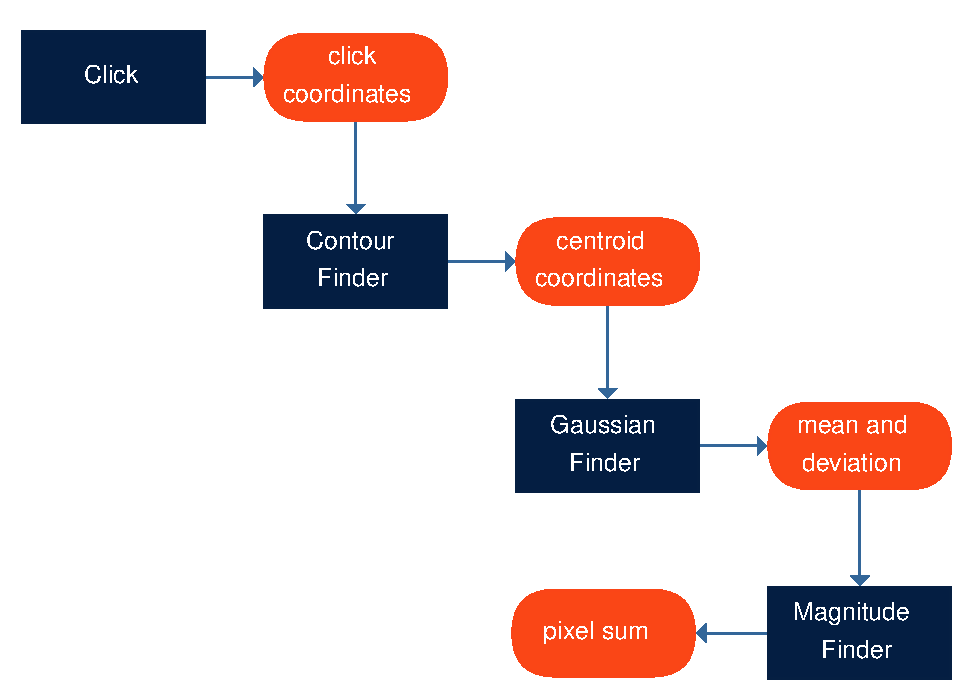
\includegraphics[width=.8\linewidth]{orange4.pdf}
	\caption{The program runs a series of functions (blue) that return specific information (orange) that is used by the following function.}
	\label{fig:flowchart}
\end{figure}

\section{Photometry}

Once an event is detected by D6, it can then be run through a script that will analyze the frames and output the desired photometric information. The script is written in Python 3, and the user can run it through the use of the accompanying graphic user interface. The interface can be seen in Figure~\ref{fig:gui}. A user simply runs the script while directing it to the location of the video they would like to analyze. The program runs through the video a single frame at a time, and loops through its functions until completing analysis on all the frames in the video.

The video processing is done through using the video read functionality of \texttt{OpenCV}. The video frames are always converted to grayscale at the beginning of the loop, so there is only one channel of pixel values instead of three that would occur with color video.

\begin{figure}[htpb]
	\centering
	\includegraphics[width=\linewidth]{ProgramLandscape.png}
	\caption{The GUI allows one to see the initial frame, and view the results all in one window.}
	\label{fig:gui}
\end{figure}

Upon running the script, the user will first see the first frame of the video. This is where the user will be required to make a selection on the screen identifying where the object and reference stars are located. The user simply left clicks on the desired object, and right clicks on a reference star of known magnitude.The user uses a slider to adjust the threshold level until both objects are clearly separated from the background. An example of a frame that a user could see is seen in Figure~\ref{fig:scene}. The user's clicks initialize the script. 

\begin{figure}[ht!]
	\centering
	\includegraphics[width=0.6\linewidth]{scene.png}
	\caption{The first frame of an event. The user clicks on this image in the GUI.}
	\label{fig:scene}
\end{figure}

\subsection{Recognizing a User's Click}

Why does the user need to click on the objects? The program needs a general idea of where the object is in question on the frame. It can follow the moving object after that, as long as it has a starting point. This is outlined in Figure~\ref{fig:clickfinder}

\begin{figure}[h!]
	\centering
	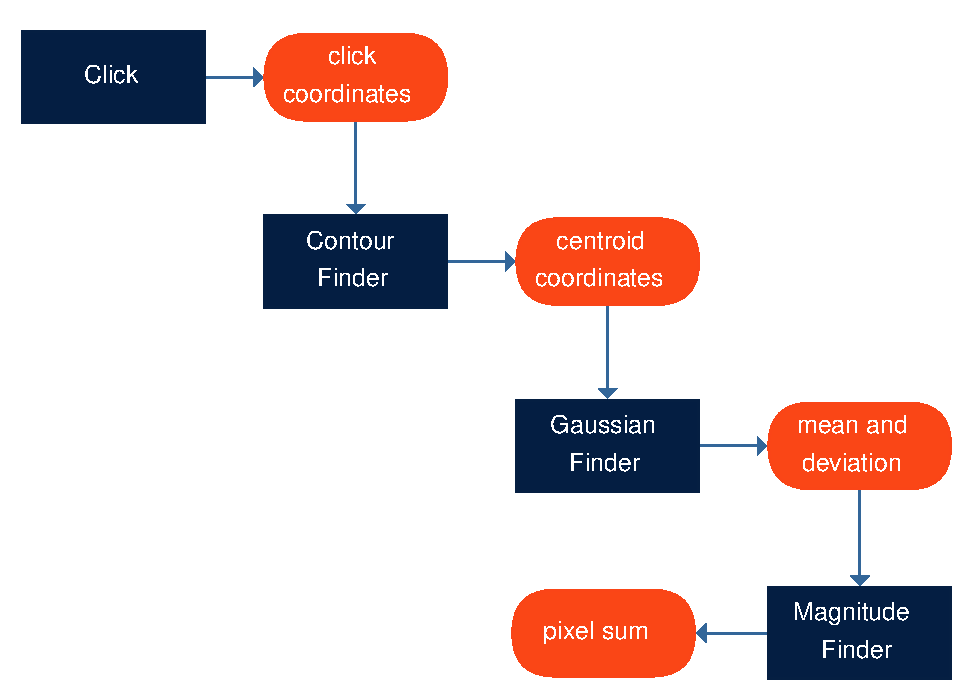
\includegraphics[width=\linewidth]{orange4.pdf}
	\caption{Each click gives crucial information for latter functions: The initial coordinates of the meteor and reference star.}
	\label{fig:clickfinder}
\end{figure}

Using the \texttt{OpenCV} computer vision python package, the coordinates of the user's clicks can be extracted and used in the script. The user's left click records the corresponding X and Y coordinates as a tuple identify as the location of the object. The user's right click records the corresponding tuple as the location of the reference star. The user can click multiple times, with each click overwriting the previous one until the user is satisfied with their click accuracy. After both objects have been selected, the program's \texttt{Run} button is selectable. The user clicks the button to run the remainder of the script.

%The location of the center of the object is done through the use of two functions: a \texttt{click} function and a \texttt{FindingMax} function. The click function allows the user to interact with the image through OpenCV. The function creates two global variables that are crucial to the activation of the other following functions: The x and y coordinates of that click. After all, without the user clicking to identify the object and the reference star, the program has nothing to analyse. These variables are tuples containing the x and y positions that were clicked. In order to differentiate the reference star and the object, different clicks were assigned to each one. A left click marks the coordinates as the location of the reference star, and a right click will mark the coordinates as the location of the fireball. The program will only record the latest clicks when the image is open; previous clicks will be overridden by the newest clicks. The program does not continue until the user exits the frame window with a key press.

\subsection{Fitting a contour to the object}
The location of the object is now set as the exact pixel the user clicked on. The user may have provided a solid estimate on where the true center is with their click, but it most likely not actually the true center. The estimate allows the program to run its algorithm to find a more accurate location of the object in the nearby vicinity of the click. The aforementioned algorithm's process is outlined in Figure~\ref{fig:contourfinder}. This more accurate object location will be necessary when the program tries to fit Gaussian fits to the data, which will be needed to identify the radius of the object.

\begin{figure}[h!]
	\centering
	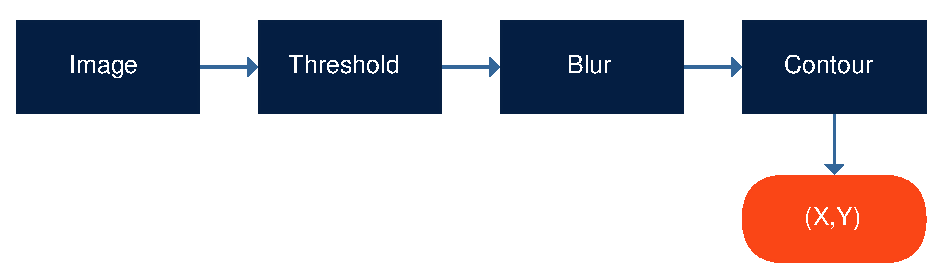
\includegraphics[width=\linewidth]{orange1.pdf}
	\caption{The steps the image is processed with to get a more accurate object position}
	\label{fig:contourfinder}
\end{figure}

The script takes the X and Y coordinates of where the user thinks the object is and isolates that part of the frame. The image is then blurred using an \texttt{OpenCV} command that blurs the edges of the pixels using a Gaussian equation to fade their light. This is done as an array of pixel values is discrete, and are not ideal to model a continuous equation, such as a Gaussian, off of. The image is then thresholded at a certain percentage. Thresholding essentially divides all pixels into a group lighter than the percentage and a group darker than the percentage. The darker pixels are all turned black, and the lighter pixels are all turned white. This, combined with the blurring, turns the object into a white round object. An example of this process can be seen in Figure~\ref{fig:ThresholdComparison}.

\begin{figure}
\centering
\begin{subfigure}{.5\textwidth}
  \centering
  \includegraphics[width=.75\linewidth]{thresholdd6zoom.png}
  \label{fig:nothresholdd6}
  \subcaption{The image before being thresholded.}
\end{subfigure}%
\begin{subfigure}{.5\textwidth}
  \centering
  \includegraphics[width=.75\linewidth]{nothresholdd6zoom.png}
  \label{fig:thresholdd6}
  \subcaption{The image after being thresholded.}
\end{subfigure}
\caption{A thresholded image, when adjusted properly, allows the program to locate an object easier.}
\label{fig:ThresholdComparison}
\end{figure}

%\begin{figure}[ht!]
	%\centering
	%\includegraphics[width=0.5\linewidth]{thresholdd6.png}
	%\caption{The fireball in a unaltered frame can sometimes be too dim for the program to detect for the entirety of the event.}
	%\label{fig:nothresholdd6}
%\end{figure}

%\begin{figure}[ht!]
	%\centering
	%\includegraphics[width=0.5\linewidth]{nothresholdd6.png}
	%\caption{A thresholded image, when adjusted properly, allows the program to locate an object easier.}
	%\label{fig:thresholdd6}
%\end{figure}

This process also has the benefit of making it easier for the user to locate the object. It is especially useful for finding the reference star, which is often much dimmer than the meteor. This is evident by no stars being visible in Figure~\ref{fig:thresholdd6}, but some being visible in Figure~\ref{fig:nothresholdd6}.

Another OpenCV command called \texttt{findContours} is implemented to find the center of that ellipse. Its algorithm is exactly like how one would find the center of mass of an object, but with the intensity of the pixel being the ``mass'' in the calculations. At this point, the program now has a much more precise idea of where the center is. With the object's coordinates updated, the thresholded frame is discarded, and the following analysis is continued with the undoctored data. 


\subsection{Fitting a Gaussian to the contour}
Now that there is an accurate object location, we can fit a Gaussian curve to the data in both the X and Y dimensions. We want to do this because having a Gaussian curve gives us a known standard deviation, and we can then calculate the radius of the event using that standard deviation. This process is outlined in Figure~\ref{fig:gaussianfinder}.

\begin{figure}[h!]
	\centering
	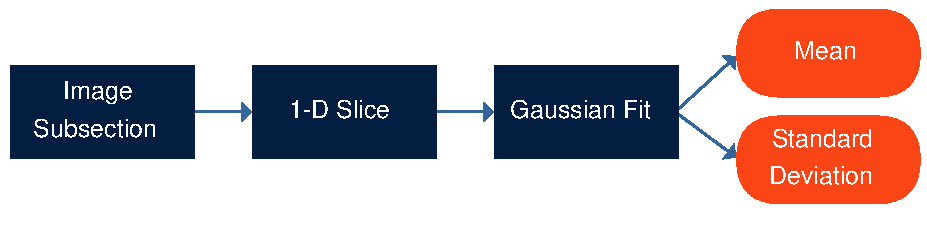
\includegraphics[width=\linewidth]{orange2.pdf}
	\caption{The steps taken to find the Gaussian parameters of the data.}
	\label{fig:gaussianfinder}
\end{figure}

The formula for a Gaussian curve is 

\begin{equation}
	ae^{-(x-x_0)^2/(2\sigma^2)}
\end{equation}
where a is the amplitude, $x$ is the point along the curve, $x_0$ is the center of the curve, and $\sigma$ is the standard deviation. A function is used from the Python library called \texttt{SciPy}\footnote{The author prefers the package to be pronounced ``skip-ee'' when discussing any matter involving this paper}. A Gaussian fitting will output a mean and standard deviation, but first the \texttt{SciPy} function needs a strong estimate of the mean to attempt to fit the data. This is why the center of the object was calculated using the contour method previous discussed. In our program, we calculate two one-dimensional Gaussian curves across that center. The function fits the Gaussian curves to 20 pixel slices centered at the point in the X and Y directions. The Gaussian curve also returns its mean, and the mean of the X slice and Y slice is updated to represent the objects location once again, which is used to fine-tune the location of the event. The clicking, contouring, and Gaussian fitting functions can be thought of as a sequence of steps to acquire the most accurate center, along with the acquisition of the standard deviation data mentioned. The curves can be plotted and saved as PNGs. The Gaussian curves of one such frame can be seen in Figure~\ref{fig:testplot}.

\begin{figure}[h!]
	\centering
	\includegraphics[width=.6\linewidth]{testplot.pdf}
	\caption{The Gaussian curves in this plot align with the image, so one can visually confirm that they are fitting the data.}
	\label{fig:testplot}
\end{figure}

Occasionally, an anomaly or poor data will make the Gaussian function unable to actually fit the data to a Gaussian curve. In this case, an exception is called in the code to just use the estimates provided as the true outputs of the Gaussian function instead of the error message. By using the estimates, the sequence of functions can continue as-is without any additional manipulation. The frame is skipped in the creation of the final light curve. This is done to ensure the program can finish to completion, and not end in the middle. If this was not implemented, the program would be break before processing the command to create the light curve. Later on, it is possible to view the data to ensure the Gaussian curves aligned well with the pixel values.

A Gaussian curve is to be expected from something such as a point light source as it dims out radially. An object will not have a definite edge: it will fade away into the background. This can be shown in Figure~\ref{fig:NoCircles} of a Gaussian fit. The Gaussian function has the benefit that its standard deviations are directly proportional to certain percentages of the data fitted to the functions. This is commonly known as the 68-95-99.7 rule: one standard deviation covers 68\% of the data, three standard deviations covers 95\% of the data, and three standard deviations covers 99.7\% of the data. After that, the diminishing returns are not enough to overcome the extra noise in our data.

\begin{figure}[ht!]
	\centering
	\includegraphics[width=.4\linewidth]{NoCircles.png}
	\caption{The object is located in the center of this slice, and its light fades radially out from that center.}
	\label{fig:NoCircles}
\end{figure}

There are few details in the calculation of the radius from the standard deviations, however. The X and Y radii are defined by multiplying their respective Gaussian curve standard deviations by two, and then rounding up to the nearest integer. While the standard deviations themselves may be decimals, the image consists of only integer values, so any other number would not be compatible. In other words, one can not sum over a fraction of a pixel; either the entire pixel is used or none of it is. The radius of the circle is then defined to be whichever of these two radii happen to be the largest. They should be the same in theory, but may vary by a pixel due to the rounding process mentioned. The pixels within this radius will be summed over in the next section. 

Why do we sum over all the pixel values inside the radius instead of just integrating over the Gaussian fit? Figure~\ref{fig:NoCircles} also provides a strong piece of visual evidence why someone wanting to just integrate over a two-dimensional Gaussian using the X and Y Gaussian slices would be oversimplifying the nuances in the data. 

First off, A Gaussian function is by definition a continuous function; that is one of the reasons it is so nice for finding the radius, all of its values are usable. However, the data itself consists of pixels, a discrete form of data. This is why the program runs the radius up to the nearest integer; one cannot sum over a fraction of a pixel. This discreteness in the data is inherently different than a continuous model, and if the sum was found off that, it would be making too many assumptions about what the data \textit{could} be instead of what it actually \textit{is}\footnote{And while some assumptions have to be made in this photometry analysis, for that reason we cannot really afford to make any superfluous assumptions}.

All of this reasoning is still making one critical assumption of the data: that it is perfectly radially symmetrical. With the actual photometric data, we can clearly see there are some fluctuations in how wide the radius is at different points. In Figure~\ref{fig:radius}, the object's appearance is stretched in the upper-left direction and in the upper half in general. This is why it is critical to remember that the Gaussian is merely an approximation used to automate the calculation of the radius. It is \textit{not} perfect, and does not represent the data well. What it does do well, however, is gives a solid representation of where the majority of the pixels are.

\subsection{Calculating the magnitude of the object}

Now all of the needed information is gathered to find the magnitude of the object at that frame. With the parameters from the Gaussian function, we know where the object is centered and, by defining its radius to be three standard deviations, we know the radius of the object. After subtracting background light, we then can sum over all the pixels within that radius to find the amount of light, or the magnitude, that our camera sees from the object.  Doing this every frame gives us the light curve of the event over time. A diagram describing this process can be seen in Figure~\ref{fig:magfinder}.

\begin{figure}[htpb]
	\centering
	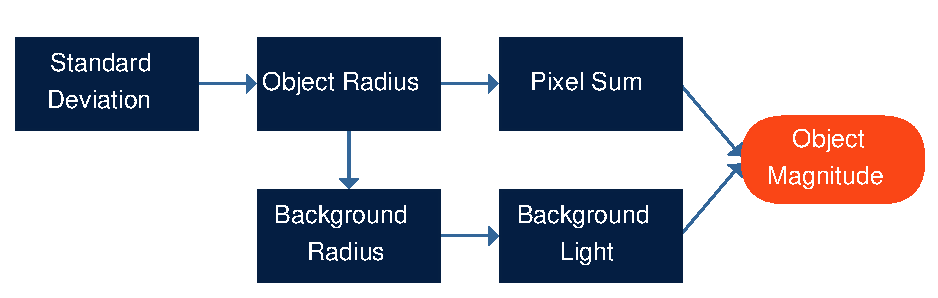
\includegraphics[width=\linewidth]{orange5.pdf}
	\caption{The steps the function goes through to find the magnitude of the object.}
	\label{fig:magfinder}
\end{figure}

The radius can give us the lengths along the axis, but not the pixels of the entire circle we are searching over. The program takes a 10 x 10 search area around the center point, and checks all the points to see if they lie inside the given radius using the distance formula. If a point is within the radius, it is appended to a list to be used later. This can be seen in Figure~\ref{fig:radius}.

\begin{figure}[ht!]
	\centering
	\includegraphics[width=0.4\linewidth]{Radius.png}
	\caption{The pixels in red are within the calculated radius for this fireball.}
	\label{fig:radius}
\end{figure}

We need to remove the background light from the calculation so we can sum over the pixel values attributed to the object's light only, not from any other source. If the background light is not subtracted the values of the pixels would be artificially elevated due to the existence of that inherent background light. To do this, we need to find a second radius of points around the circle that can be used to determine the average value of the background light. The background light can be somewhat noisy, so that is why we take an average of a group of background pixels. The pixels in question are chosen by finding pixels within a radius of the object's radius + 10 pixels, not including the pixels inside the object's radius. This creates a ring around the object's radius, as shown in Figure~\ref{fig:background}. In theory, if the Gaussian-based radius is too large, the background light subtraction will mitigate that overestimate.

\begin{figure}[ht!]
	\centering
	\includegraphics[width=0.4\linewidth]{BackgroundRing.png}
	\caption{The pixels in yellow are the values being used to find the average background value. The object can be seen inside the yellow ring.}
	\label{fig:background}
\end{figure}

One problem that occasionally happens is the background search radius will go beyond the actual size of the image. This problem occurs when an object gets close to the sides of the image. In order to prevent this, and crashing the program, a loop goes through the pixel indices in the background list and checks to make sure they are not greater than the dimensions of the image. If any are, they are ignored. 

There is also a two pixel buffer between the two areas for extra wiggle room. This is important due to the conversion to integers when finding the two radii. The radii are not perfect circles, as while the distance may be in the middle of a pixel, you can not just split a pixel. Both of the radii calculations round up, and take that whole pixel, which could create a pixel on the edge of the background radius and the object radius being used in both summations if there was not a buffer zone.This is easily seen when both the object's radius and the background ring is displayed on the same picture, such as in Figure~\ref{fig:BothCircles} 

\begin{figure}[ht!]
	\centering
	\includegraphics[width=0.4\linewidth]{BothCircles.png}
	\caption{The pixels in orange are within the object's radius. The yellow pixels are the background ring. The gray area in-between is the buffer.}
	\label{fig:BothCircles}
\end{figure}

The program then sums all the pixel values in the list of values that were within the inner radius. This is done through a for loop that adds the value onto itself with every iteration through the list, while subtracting the average background magnitude from each individual point. This is the raw measurement of light from our specific camera.

Cameras have different sensitivities, so there is an offset that needs to be accounted for to have our specific camera be able to calibrate to the standard units of magnitude.   This is then entered into Equation~\ref{equation:instrument} to find the instrumental magnitude. 

\begin{equation}
	M_I = -2.5 \log_{10}\left( \sum \text{pixels}\right) + \text{offset}
	\label{equation:instrument}
\end{equation}

This is the same equation from the previous section. The offset can be calculated by Equation~\ref{equation:offset}

\begin{equation}
	\text{offset} = M_I - M_C
	\label{equation:offset}
\end{equation}
where $M_I$ and $M_C$ are the instrumental magnitudes and catalog magnitudes of the same object.

This is why a reference star is needed. The object in question, the fireball, does not have a catalog magnitude, but the reference star does. This calculates the offset for the camera, which then can be applied to equation~\ref{equation:offset} for the fireball. This offset is calculated as an average over the entire event. The average is calculated due to the small amount of fluctuation each frame may have in their offsets due to variables such as atmospheric distortion or haze.

The program runs the previously mentioned functions for every frame in the video, and loops through this process until the video is completed. This overview can be seen in Figure~\ref{\fig:moreflow}.

\begin{figure}[ht!]
	\centering
	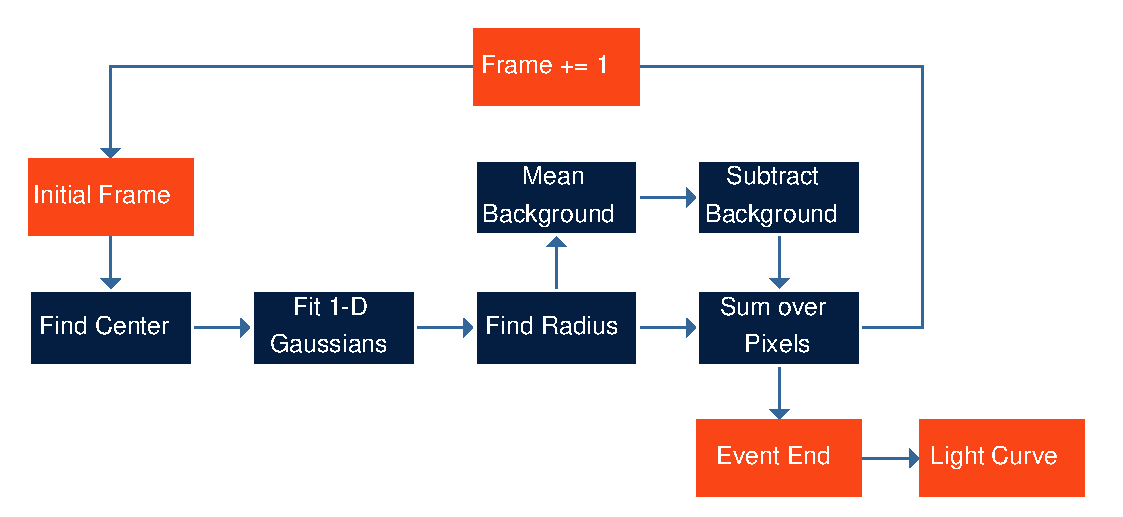
\includegraphics[width=\linewidth]{largeorange.pdf}
	\caption{The program loops over most of the previous functions for each event.}
	\label{fig:moreflow}
\end{figure}

In order to successfully loop through the frames, there needs to be a way for the program to jump from the center of one frame to the center of the next. The process of calculating a more precise center through each function allows the program to adjust the previous frame's center to the next frame's center without any difficulty, as the amount of pixels the center of the object appears to travel in each frame is usually no farther a distance than the average user's click is from the actual event for the first frame. This process is shown in Figure~\ref{\fig:updatingxy}

\begin{figure}[htpb]
	\centering
	\includegraphics[width=0.5\linewidth]{flowlast.png}
	\caption{The updating process of the values used as the object's coordinates}
	\label{fig:updatingxy}
\end{figure}

PNGs of each frame's Gaussian fits along with the visualization of the radii are optional through the loop. If enabled, the result is exactly like Figure~\ref{fig:testplot}. If this is enabled, the program may take up to 30 seconds to run, as it is memory intensive to save hundreds of PNGs. If it is disabled, the program finishes within a second.





\chapter{Data}

There are 3 types of data we can use to test the capability of the script. Iridium flares can be predicted before hand, allowing one to prepare to collect their data. NASA data provide a steady source of fireball events to access along with their data to compare to. Finally, fireball events detected by D6 will be tested, 

\section{Iridium Flares}

The next step in testing out the script is to run it in conjunction with video collected directly from D6. A simple way to do this is to run it against a video clip of an iridium flare that D6 captured. There are two benefits of testing against an iridium flare. First, iridium flares are monitored online and their max magnitudes are recorded. We can find the maximum value from our light curve and compare it to that maximum magnitude. Second, the light curves from iridium flares are very smooth. This makes it easy to notice any discrepancies in individual frames. We have collected two iridium flare events using D6. 

On *some date in fall*, D6 was able to capture an iridium flare going over Collins Hall at Willamette University in Salem, Oregon. The first frame of this event is shown as Figure~\ref{fig:iridium}. 

\begin{figure}[ht!]
	\centering
	\includegraphics[width=0.6\linewidth]{iridium.png}
	\caption{The first iridium flare captured by D6 at Willamette University.}
	\label{fig:iridium}
\end{figure}

The event was analyzed by the script, producing an accurate-looking light curve. This is shown in Figure~\ref{fig:iridiumcurve}

\begin{figure}[ht!]
	\centering
	\includegraphics[width=0.6\linewidth]{/home/luke/Data/IridiumFlare/IridiumMag.pdf}
	\caption{Name}
	\label{fig:iridiummag}
\end{figure}

\begin{figure}[ht!]
	\centering
	\includegraphics[width=0.6\linewidth]{/home/luke/Data/IridiumFlare/IridiumCurve.pdf}
	\caption{The light curve of the iridium flare event.}
	\label{fig:iridiumcurve}
\end{figure}

The first thing to check is if it qualitatively agrees with visual inspect of the event's video. The iridium flare's brightness seems to dramatically increase before dimming away. Both Figure~\ref{fig:iridiumcurve} and Figure~\ref{fig:iridiummag} agree with that assessment. So in a general sense, the photometry program is capable of following the event.

Some issues did emerge from this event, however. Ideally, we would like to be able to compare the maximum magnitude from the light curve our program created to the recorded maximum magnitude of the event. Unfortunately, the iridium flare was so bright that it oversaturated our camera. This can be seen in Figure~\ref{fig:ObjectPlot055}.

\begin{figure}[ht!]
	\centering
	\includegraphics[width=0.6\linewidth]{ObjectPlot055.png}
	\caption{ObjectPlot055}
	\label{fig:ObjectPlot055}
\end{figure}

Figure~\ref{fig:ObjectPlot055} allows us to see that the center of event is too bright for our camera's sensors. As a result, we are unable to find the current maxium magnitude of that iridium flare event. This saturation also explains why the peaks in Figure~\ref{fig:iridiumcurve} and Figure~\ref{fig:iridiummag} last for a substantial portion of the event; the true peak brightness isn't visible on those graphs. 

Another issue that is apparent in the iridium flare data is an excess of noise insections of the data. Specifically, the noise at the end of the event appears most jarring in Figure~\ref{fig:iridiummag}. When the event nears its end, the signal to noise greatly decreases. This noise is a result of the background light that has already been mentioned. Since the event is at its end, it is becoming incredibly dim, and in its last moments its signal is basically equal with the background light around it. Since the background light value we are using is the average of the area around the event, there arises occasions where the pixels of the event are smaller than the background light at this stage. This creates a magnitude that is the resultant of a log of an incredibly small, or even negative number. Since taking the logarithm of a negative error would break the program if left untreated, those values are set to 0. So, at the end of an event before the program no longer detects any trace, it has a few data points that are incredibly smaller, whose tiny size is magnified (this seems oxymoronic???) in the logarithmic-based light curve. While not aesthetically pleasing, this small values do not affect our results, as our results will be based off integrating the intensity along the light curve.

\section{Comparison to NASA Data}

The previous section provided an example of an acquired light curve from the completion of analysis from a NASA video clip. By running the script against clips from NASA, we can confirm that the script is working by comparing it to NASA's light curves provided with the videos. Examples of this are discussed below.

When it is finished, the end result is the magnitude of each frame plotted over the time of the event, showing the light curve of the event. An example of this can be seen in Figure~\ref{fig:lightcurve}. 

\begin{figure}[htpb]
	\centering
	\includegraphics[width=0.6\linewidth]{/home/luke/Data/NASA/2018-03-21-0814/MeteorCurve.pdf}}
	\caption{A lightcurve the program calculated off one of NASA's detected meteor events.}
	\label{fig:lightcurve}
\end{figure}


The general trend shows that program's methodology in calculating the magnitude is sound. We would expect the brightness to gradually grow before diminishing again, and the graph agrees with that. This event in question was detected off from one of NASA's cameras. As a result, we can compare our light curve to NASA's to double check. NASA's light curve can be seen in Figure~\ref{fig:nasa}. They are pretty similar.

\begin{figure}[ht!]
	\centering
	\includegraphics[width=0.6\linewidth]{/home/luke/Data/NASA/2018-03-21-0814/201803210814.pdf}
	\caption{The event in question is the light curve on the top.}
	\label{fig:nasa}
\end{figure}


\section{Fireballs detected with D6.}

Ultimately, however, the goal of our research is to show our all-sky camera's capabilities. The final test of the photometry script is thus the ability for it to detect new data collected from our own all-sky camera. With self-collected data, however, there are often problems that need to be troubleshooted. One problem that emerged early on in our desire to build an ultra compact and affordable unit was that our hardware was not fast enough to write the frames of the events to the harddrive cleanly. The result of this is incomplete video frames, creating gaps in the data. This can be seen in Figure~\ref{fig:D6Glitch}. 

\begin{figure}[ht!]
	\centering
	\includegraphics[width=0.6\linewidth]{D6Glitch.png}
	\caption{The incomplete frame data can be seen in both slices of the pixel data.}
	\label{fig:D6Glitch}
\end{figure}

This results in frames with much lower pixel values inside the object's radius than what one would expect, and what it would be if accurately representing the meteoritic phenomenon correctly. This is further seen in the resulting light curve, show in Figure~\refPfig:{D6LightCurve}.

\begin{figure}[ht!]
	\centering
	\includegraphics[width=0.6\linewidth]{/home/luke/Data/D6/D6Curve.pdf}
	\caption{The light curve of this event is much less smooth than one would expect from a fireball}
	\label{fig:D6LightCurve}
\end{figure}

\chapter{Conclusion}

So what does the data show us regarding the current capabilities of our all-sky camera setup? There are improvements to be made, problems to troubleshoot, but on a wholistic sense, the system is most assuredly capable of photometrically analyzing the events.

\section{Critique}
One potentially problematic issue is there is no current way for us to compare our calibrated light curves to other calibrated magnitudes. Each of the potential ways to do so are somewhat flawed in one aspect or the other. Comparing our data to NASA's allows us to effectively see if the shape of our light curve is accurate, but as their posted data is uncalibrated to a reference object, we cannot confirm our calibration is right then either. The other source of comparison is the Iridium flare data. The Iridium flare data does not have light curves to compare to but they do have posted maximum magnitudes. Unfortunately, as mentioned in the data section, our camera cannot see that maximum magnitude in most Iridium flare events due to oversaturation. For future events, it would be worthwhile to attempt at adjusting the sensitivity levels of the camera. The only other option would be extrapolating the peaks from the Gaussian curves, but that creates more accuracy issues as previously mentioned.

In order to confirm our calibration is accurate, we should find data sets with calibrated magnitudes and posted video clips to compare to. However, it is worth noting that if the program can detect the shape of the light curve accurately, which it has repeatedly shown it can, it should have no problem with the calibration. After all, the calibration is dependent on the same algorithm, only it arises from the calculation of the reference star's magnitude instead of the object's magnitude. In fact, it should be even easier to do so, as the reference star does not move throughout the duration of the event; the program does not need to update the position it is covering. 

There is also potentially more data to gain from the reference objects as well. As mentioned in the Chapter 4, there are often multiple reference objects seen in the video. Calibrating off of multiple reference objects would give us greater confidence in the calibration capabilities. As those objects' magnitudes should be constant throughout the event, their light curves could also allude to the margin of error in our light curves depending on how nonlinear their light curves appear.

\subsection{Atmospheric Extinction}
Further examination is needed to figure out whether or not the discrepancies at the beginning of the light curve is based off a correctable parameter such as atmospheric extinction, or whether it arises from a systematic failure in the program to successfully find the magnitudes of dimmer objects.

We most likely will have to account for atmospheric extinction. Atmospheric extinction, visualized in \ref{fig:extinction}, is a phenomenon caused by different areas of the sky having different amounts of air between them and the observer. As a result, a meteor near the horizon is separated by more air, and thus appears dimmer than if the same meteor was right above the observer. 
\begin{figure}[ht!]
	\centering
	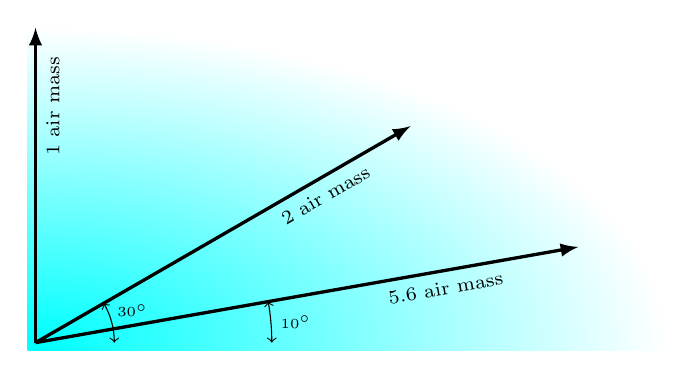
\begin{tikzpicture}
		\clip (-.1,-.1) rectangle (8,4);
		\shade[inner color=cyan, outer color=white] (0,0) ellipse (8cm and 4cm);
		\draw[-latex, very thick] (0,0) -- (90:4) node[near end, font=\scriptsize, sloped, below]{1 air mass};
		\draw[-latex, very thick] (0,0) -- (30:5.5cm) node[near end, font=\scriptsize, sloped, below]{2 air mass};
		\draw[-latex, very thick] (0,0) -- (10:7cm) node[near end, font=\scriptsize, sloped, below]{5.6 air mass};
		\draw[<->] (0,0) ++(1,0) arc (0:30:1) node[pos=.8, right, font=\tiny]{$30^{\circ}$};
		\draw[<->] (0,0) ++(3,0) arc (0:10:3) node[midway, right, font=\tiny]{$10^{\circ}$};
	\end{tikzpicture}	
	\caption{There is more air in between someone and an object along the horizon than an object straight above them.}
	\label{fig:extinction}
\end{figure}


\section{Outlook}
This project is far from being completed. Creating a program that appears to successfully analyze meteor events is the most important building block for collecting data, but there is much more to do beyond that. Now that the script is set up, a substantial amount of events would need to be collected with our own all-sky camera to be able to make any reasonable conclusions about the near-Earth population. If we are able to do so, we are then able to show that a setup similar to D6 is a viable alternative to the larger setups currently in place.  The data that is needed to be collected is the photometric data of the events, but there is substantial statistical analysis that needs to be done to extrapolate that photometric data into meteor size. The future of this project is thus based on optimizing the data collected and performing data analysis on that data to justify drawing any reasonable conclusion from the collection of individual events.

\appendix

\chapter{Code}

\section{Photometry Script}
\inputminted{python}{/home/luke/Git/allsky/Photometry.py}

\section{GUI Script}
\inputminted{python}{/home/luke/Git/allsky/PhotometryGUI.py}


%\bibliographystyle{urcsbiblio}
\bibliographystyle{amsalpha}
\bibliography{Bibliography}

\appendix
%\include{notebook}

\end{document}
